\documentclass[12pt]{article}
\usepackage{enumitem}
\usepackage{graphicx}
\usepackage{geometry}
\usepackage{physics}
\usepackage{tikz}
\usetikzlibrary{calc,backgrounds}
\usepackage{amsthm,mdframed,hyperref}
\usepackage{amssymb}
\usepackage{amsfonts}
\usepackage{epigraph}
\usepackage{booktabs, tabularx, array}
\usepackage{longtable}

\newtheorem*{principle}{Principle}
\newtheorem{definition}{Definition}
\theoremstyle{plain}

\newtheorem{theorem}{Theorem}
\newtheorem{lemma}{Lemma}
\newtheorem{corollary}{Corollary}
\newtheorem{remark}{Remark}

\newcommand{\gammarel}{\gamma_{\!\mathrm{rel}}}
\newcommand{\stick}{s_{\mathrm{tick}}}


\newcolumntype{Y}{>{\raggedright\arraybackslash}X}

\newtheorem{innerTakeaway}{Takeaway}
\newenvironment{takeaway}[1][]{
  \begin{mdframed}[linewidth=0.6pt,roundcorner=4pt]
  \begin{innerTakeaway}[#1]\label{takeaway:universal–flow}
}{\end{innerTakeaway}\end{mdframed}}

\usetikzlibrary{decorations.pathmorphing, arrows.meta, positioning}

\title{Universal Time and Tick Suppression: A Realist Interpretation of Relativistic Effects}
\author{Dickson Terrero}
\date{\today}

\begin{document}

\maketitle
\begin{abstract}
We present a realist reinterpretation of relativistic phenomena, \emph{Universal Time and Tick Suppression}. Time is taken not as an observer–relative parameter but as a universal, dynamic axis: a smooth future–directed timelike field \(U\) along which the total mass–energy of the universe advances. Effects usually described as “time dilation” are recast as \emph{tick suppression}: a physical slowing of internal processes (clocks, decays) due to the energy cost of sustaining motion through space or persisting in gravitational fields. This energy–allocation mechanism is formalized as the \emph{Inertial Suppression Principle}, providing a causal reading that is operationally equivalent to standard relativity while ontologically distinct. We also specify a light–based calibration of duration, using local MCIFs and \(c\), that is independent of potentially suppressed clocks. The framework unifies kinematic and gravitational slowdowns under a single mechanism, preserves all empirical predictions, and offers a clear, absolute (yet physical) notion of time that clarifies puzzles of simultaneity without altering relativistic phenomenology.
\end{abstract}

\section*{Introduction}

Special relativity provides a complete and remarkably successful account of local temporal and spatial measurements: time, length, and simultaneity are all dependent on an observer's state of motion~\cite{Einstein1905}. However, because simultaneity is frame–dependent, SR does not define a universal present across cosmic distances; each observer reconstructs only a \emph{local} now. This presents a foundational challenge. On quantum scales, entanglement exhibits nonlocal correlations that, while obeying no–signalling theorems, sit uneasily with SR's purely local, frame–relative simultaneity. This motivates a re–examination of the global structure of time.

\medskip
\noindent
This paper presents a realist reinterpretation of relativistic phenomena, \textbf{Universal Time and Tick Suppression}, that restores a global present without altering any of the tested predictions of relativity. The framework is built on three core principles:
\begin{itemize}
    \item There is one shared, objective reality.
    \item There exists one universal time, anchored in the observable structure of the cosmos.
    \item Relativistic effects are real, physical suppressions of process rates, not changes in the flow of time itself.
\end{itemize}

\medskip
\noindent
The central thesis is that \textbf{processes slow down, not time}. We propose a universal time coordinate $T$ whose level sets, $\Sigma_T$, define a shared cosmic present. Effects commonly known as "time dilation" are reinterpreted as "tick suppression," a physical reduction in the rate of internal processes (clocks, particle decays) for any system not comoving with the universal time flow.

\medskip
\noindent
The paper is structured as follows. Section~\ref{sec:geometric-structure} introduces the core geometric picture and conceptual framework. Section~\ref{sec:time-moment-duration} then lays out the complete mathematical formalism. We anchor the theory in observable cosmology in Section~\ref{sec:cosmological-anchoring}, a choice justified by the Principle of Global-Local Decoupling (Section~\ref{sec:principle-global-decoupling}). The central physical mechanism of tick suppression is detailed in Section~\ref{sec:mechanism}. Subsequent sections apply the framework to compare the theory to alternative interpretations (Section~\ref{sec:comparison-with-LET}), resolve the problem of simultaneity (Section~\ref{sec:simultaneity}), and solve the classic Twin Paradox (Section~\ref{sec:twin-paradox}), before we present our concluding arguments in Section~\ref{sec:discussion}.

\section{The Geometric Structure of Cosmic Time}
\label{sec:geometric-structure}
This interpretation posits a fundamental, geometrically explicit universal time axis, denoted by the parameter $T$. This parameter foliates spacetime into hypersurfaces of constant cosmic time. This foliation is not arbitrary but is defined by the congruence of worldlines representing the flow of the universe's total mass–energy content, described by a smooth, future–directed timelike 4–velocity field $U^\mu$~\cite{Carroll2004}.

\subsection{Time as a Dynamic Axis}
Time is the universe’s dynamic axis: a physical direction in spacetime, anchored at the agreed start $(O,\Sigma_0)$, along which all mass–energy evolves~\cite{Rindler2006}.

\medskip
\noindent The relationship between this universal time and local spatial dimensions can be intuitively visualized through a Euclidean analogy. Consider the vector representing the direction of temporal advancement in a 3D space:
\[
\vec{T} = (1,1,1).
\]
This vector is equally inclined to the $x$, $y$, and $z$ axes. The angle $\theta$ between $\vec{T}$ and any spatial axis is given by:
\[
\cos \theta = \frac{\vec{T} \cdot \hat{x}}{|\vec{T}|} = \frac{1}{\sqrt{3}} \quad \Rightarrow \quad \theta = \arccos\left(\tfrac{1}{\sqrt{3}}\right) \approx 54.7^\circ.
\]

\paragraph{Interpretation.}
This diagonal vector is a metaphorical illustration of the timelike direction $U^\mu$ orthogonal to the cosmic time foliation. \emph{This analogy is purely illustrative; no preferred spatial axes are implied.} It symbolizes that the progression of cosmic time is a global property that exerts a fundamental influence on all local spatial dimensions, without implying a privileged spatial frame. The physical reality is the 4–velocity field $U^\mu$ and the foliation it defines, not a literal diagonal in a Euclidean space.

\newpage

\begin{figure}[h]
    \centering
    \begin{tikzpicture}[scale=1.05, >=stealth,
      axis/.style={->,thick,white},
      guide/.style={dashed,thin,gray!60},
      gridl/.style={line width=0.2pt, draw=gray!35},
      background rectangle/.style={fill=black},
      show background rectangle]

      %---------------- Base coordinates ----------------
      \coordinate (O)    at (0,0);            % origin
      \coordinate (Xend) at (5.6,0);          % x axis tip
      \coordinate (Yend) at (0,4.1);          % y axis tip
      \coordinate (Zend) at (4.9,-2.1);       % z axis tip
      \coordinate (Tend) at (3.9,2.3);        % T axis tip (red)

      %---------------- Faint base grid (minimal) -------
      \foreach \t in {0.9,1.6,2.3,3.0,3.7,4.4}{
        \draw[gridl] ($(O)!\t/5.6!(Xend)$) -- ++($(Zend)-(O)$);
      }
      \foreach \t in {0.8,1.5,2.2,2.9,3.6}{
        \draw[gridl] ($(O)!\t/4.9!(Zend)$) -- ++($(Xend)-(O)$);
      }

      %---------------- Axes ----------------------------
      \draw[axis] (O) -- (Xend) node[right] {$x$};
      \draw[axis] (O) -- (Yend) node[above] {$y$};
      \draw[axis] (O) -- (Zend) node[right] {$z$};
      \draw[axis,red, line width=1.35pt] (O) -- (Tend) node[right, white] {$T$};

      % Origin label
      \fill[white] (O) circle (2pt);
      \node[anchor=north east, align=right, text=white] at ($(O)+(-0.06,0.36)$) 
      {$(O,~\Sigma_0)$\\(Agreed start)};

      %---------------- Points along T ------------------
      \coordinate (Eearly) at ($(O)!0.32!(Tend)$);
      \coordinate (E)      at ($(O)!0.70!(Tend)$);

      % Guides from current position
      \coordinate (Ex) at (2.0,0);   
      \coordinate (Ey) at (0,1.4);   
      \coordinate (Ez) at (2.0,-0.9); 
      \draw[guide] (E) -- (Ex);
      \draw[guide] (E) -- (Ey);
      \draw[guide] (E) -- (Ez);

      % Blue U arrow (slightly steeper than T)
      \draw[->, line width=0.8pt, green!70!cyan]
        ($(E)+(-0.8,-0.9)$) -- ($(E)+(-0,-0.4)$) node[below, xshift=-9pt, yshift=-8pt, text=white] {$U$};

      %---------------- Spheres (Universe markers) ----------
      \node at (E) {\includegraphics[width=1.6cm]{images/galaxy6.png}};
      \node at (Eearly) {\includegraphics[width=0.9cm]{images/galaxy6.png}};

      \node[align=left, anchor=south west, text=white] 
        (earlyLabel) at ($(Eearly)+(-1.2,1.2)$) {\scriptsize The Universe\\[-5pt]\scriptsize at an earlier moment};
      \draw[->, thick, white] (earlyLabel.south) -- ($(Eearly)+(-0.1,0.15)$);

      \node[align=left, anchor=south west, text=white] 
        (currentLabel) at ($(Eearly)+(2.2,0.4)$) {\scriptsize Current moment\\[-5pt]\scriptsize of the universe};

      % \node[anchor=west, text=white, align=left] at ($(E)+(0.7, 0.2)$) {Current universe};

    \end{tikzpicture}
    \caption{The universal time axis $T$ represents the trajectory of the universe's total mass–energy. The red line denotes cosmic time~\cite{Minkowski1908}, flowing from the physical start $\Sigma_0$. Each galaxy represents the state of the entire universe at a specific moment on the cosmic timeline. This model treats ``earlier universe'' and ``universe now'' as distinct states along a single, objective timeline, not as frames in a relative perspective.}
    \label{fig:t–axis}
\end{figure}

\noindent This model fundamentally reorients the view of time: “earlier universe” and “universe now” are not different frames of reference, but distinct states along a single, objective timeline governing the entire cosmos~\cite{Mermin1984}.

\subsection{The Common–Now Thesis}
\label{sec:simultaneity}
The framework posits a universal foliation ${\Sigma_T}$ of spacetime, such that any two events residing on the same hypersurface $T = \text{const}$ are \emph{ontologically simultaneous}. This asserts a objective, global "now" and rejects the notion that simultaneity across cosmological distances is merely conventional or frame–dependent. It favors a view of the universe as a sequence of global states over a purely causal, sequential ordering of events.

\paragraph{Illustration of a Cosmic State}
Consider the hypersurface corresponding to the cosmic time $T \approx 13.8~\mathrm{Gyr}$:
\begin{itemize}\itemsep2pt
\item On Earth, a person reads a paper.
\item In the Andromeda Galaxy, a massive star undergoes gravitational core collapse.
\item In a distant quasar, plasma accretes onto a supermassive black hole.
\end{itemize}
Within this framework, these three events, though causally disconnected and spacelike–separated, are ontologically simultaneous – they collectively constitute part of the state of the universe at that universal time.

\paragraph{Operational Concealment of the Common Now}
This global simultaneity is operationally hidden from local observers. All measurements are made with instruments whose fundamental processes – clock ticks and rod lengths – are subject to suppression and contraction effects that depend on the observer's state of motion and gravitational environment. Consequently, different observers will \emph{reconstruct} different sets of events as being "simultaneous," perfectly matching the predictions of Special and General Relativity. This framework does not alter these empirical results; it provides a underlying reality – the foliation ${\Sigma_T}$ – of which the frame–dependent simultaneities of standard relativity are seen as perspective–dependent \emph{measurements}.

\paragraph{Empirical Anchor in Cosmology}
The postulate is empirically guided by modern cosmology. The foliation $\Sigma_T$ is identified (to a high approximation) with the hypersurfaces of statistical homogeneity and isotropy, as defined by the Cosmic Microwave Background (CMB) rest frame. This provides a non–arbitrary, operational procedure for selecting the privileged foliation, aligning it with standard \emph{cosmic time}.


\section{Time, Moment, Interval, and Duration}
\label{sec:time-moment-duration}
\subsection{Conceptual Definitions}

A central pillar of this framework is the rigorous distinction between the often–conflated concepts of \emph{time}, \emph{moment}, and \emph{duration}. Before presenting the mathematical formalism, we fix terminology:

\begin{itemize}
  \item \textbf{Time} ($T$) answers ``when?''. Operationally, it is the scalar field that orders events. Physically, its level sets $\Sigma_T$ foliate spacetime; on any open domain where the mass–energy flow $U$ is hypersurface–orthogonal, $U$ is the future–directed unit normal to these slices (i.e., $U[T]=1$).
  \item A \textbf{Moment} is a specific event in the universe, a point in both space and time.
    \begin{itemize}
      \item \textbf{Space} $(x,y,z)$ are the three coordinates that tell us \emph{where} the event happens.
    \end{itemize}
    Together, these four coordinates $(T,x,y,z)$ uniquely identify a single moment in the four–dimensional continuum of spacetime.
  \item \textbf{Universal Time Interval} is the fixed and absolute length along the universal time axis ($T$) between an agreed starting moment and an agreed ending moment.
  \item \textbf{Duration} is the comparison of how long a process unfolds relative to the invariant propagation of light within the same universal time interval; it is the answer to ``how long?''.
\end{itemize}

\subsection{Mathematical Formalism}

Let spacetime be a time–orientable Lorentzian manifold $(\mathcal{M}, g)$~\cite{Carroll2004}.

\begin{remark}[Scope]
All statements hold on a domain $\mathcal{U}$ that is globally hyperbolic with sufficiently small vorticity so that the mass–energy congruence $U$ is hypersurface–orthogonal to $\{\Sigma_T\}$.
\end{remark}

\paragraph{Notation.}
\begin{itemize}
  \item $\gamma(v) = \dfrac{1}{\sqrt{1 - v^2/c^2}}$: Lorentz factor from Eulerian 3–speed.
  \item $\gammarel = -u^\mu n_\mu \geq 1$: The general, covariant gamma factor; reduces to $\gamma(v)$ in the appropriate frame.
  \item $\alpha = \gammarel^{-1} \in (0,1]$: The relativistic conversion coefficient (ideal ``ticks per unit $T$'').
  \item $S = \dfrac{N}{\gammarel}\; s_{\mathrm{tick}}(\mathcal{C})$: The total suppression factor, including the gravitational lapse $N$ and the device factor $s_{\mathrm{tick}}$.
\end{itemize}

\begin{definition}[Time]
A (universal) \textbf{time field} is a smooth scalar $T:\mathcal{M}\to\mathbb{R}$ whose gradient $\nabla_\mu T$ is timelike and future–pointing on an open domain $\mathcal{D}\subseteq\mathcal{M}$. The level sets
\begin{equation}
\Sigma_T := \{\, p \in \mathcal{D} \mid T(p)=\mathrm{const}\,\}
\label{eq:SigmaT}
\end{equation}
foliate $\mathcal{D}$ into hypersurfaces of constant universal time.
\end{definition}

\begin{definition}[Cosmic flow field]
A smooth, future–directed time–like unit vector field $U^\mu$ on $\mathcal{D}$ represents the mass–energy congruence, chosen so that $U[T]=1$. MCIF$(U)$ denotes a momentarily comoving inertial frame of $U$.
\end{definition}

\begin{remark}
The universal time coordinate $T$ is not an abstract parameter but is physically anchored to the single, ongoing transformation of the universe. All systems and observers share the same advance $dT$ between two slices $\Sigma_{T}$ and $\Sigma_{T+dT}$, which underwrites its observer–independent character. This distinguishes it from the path–dependent proper duration $d\tau$, which measures the internal evolution of a specific subsystem~\cite{lorentz1952}.
\end{remark}

\begin{definition}[Moment (Event)]
A \textbf{moment} is an event $p\in\mathcal{M}$, uniquely identified in coordinates adapted to the foliation by $(T(p),\vec{x}(p))$.
\end{definition}

\begin{definition}[Universal Time Interval]
On a domain $\mathcal{D}\subseteq\mathcal{M}$ admitting the $T$–foliation, for $p_1=(T_1,\vec{x}_1),\,p_2=(T_2,\vec{x}_2)\in\mathcal{D}$ with $T_2\ge T_1$,
\begin{equation}
\Delta T(p_1,p_2)=T_2-T_1\ge 0,\qquad |\Delta T|=|T_2-T_1|
\label{eq:DeltaT}
\end{equation}
$\Delta T$ is path–independent and depends only on $T_1,T_2$ (not on spatial positions).
\end{definition}

\begin{definition}[Duration (light–based calibration)]
We define duration without relying on physical clocks, using light propagation as the universal invariant~\cite{Einstein1905,Rindler2006}:

\begin{enumerate}
    \item Fix the universal foliation via $T$ (with $U[T]=1$, $T|_{\Sigma_0}=0$). Choose two events $S$ and $E$ on the same $U$ flow line, with $T_S:=T(S)$ and $T_E:=T(E)$.
    \item Along that worldline, in each local MCIF$(U)$, a co–located light pulse satisfies $dt_{\mathrm{MCIF}} = d\ell_{\mathrm{light}}^{\mathrm{MCIF}}/c$.
    \item \textbf{Calibration of $T$.} We affinely fix $T$ so that along $U$,
    \begin{equation}
    dT \;\equiv\; \frac{d\ell_{\mathrm{light}}^{\mathrm{MCIF}(U)}}{c}\,,
    \quad\Rightarrow\quad
    \Delta T(S,E)=\int_{T_S}^{T_E}\frac{d\ell_{\mathrm{light}}^{\mathrm{MCIF}(U)}}{c}.
    \label{eq:calibration}
    \end{equation}
    Thereafter we use $dT$ as the universal duration unit.
    \item For any timelike worldline $\gamma$ and a clock $B$ carried along it,
    \begin{equation}
    \Delta\tau_B
    \;=\;
    \int_{T_S}^{T_E} S(\gamma)\, dT
    \;=\;
    \int_{T_S}^{T_E} \alpha(v,\Phi)\; \stick(\gamma)\; dT
    \;\le\; \Delta T(S,E),
    \label{eq:duration}
    \end{equation}
    where $\alpha(v,\Phi)\in(0,1]$ is the kinematic/gravitational conversion coefficient (where $v$ is the 3-velocity measured by the $T$–adapted orthonormal triad), and $\stick(\gamma)\in(0,1]$ is a device/material factor.
\end{enumerate}
\end{definition}

\begin{remark}[Device factor]
The factor $\stick(\gamma)\in(0,1]$ models non–relativistic imperfections of a physical clock. An \emph{ideal} atomic clock has $s_{\mathrm{tick}}=1$, so $S=\alpha$ and the reading reflects only relativistic suppression. Unless otherwise stated, we set $s_{\mathrm{tick}}=1$ in derivations.
\end{remark}

\noindent\textbf{Remarks.}
(i) The calibration is local and valid in curved spacetime.
(ii) Light provides the invariant upper bound for duration: for timelike motion, $d\tau\le dT$.

\medskip
\noindent The suppression factor is thus
\begin{equation}
S(\gamma):=\frac{d\tau}{dT}=\alpha(v,\Phi)\; \stick(\gamma)\in[0,1],
\label{eq:Suppression}
\end{equation}
and the total reported duration over $[T_{\mathrm{start}},T_{\mathrm{end}}]$ is
\begin{equation}
\Delta \tau_{\mathrm{clk}}(\gamma)
= \int_{T_{\mathrm{start}}}^{T_{\mathrm{end}}}
   \alpha(v,\Phi)\;\stick(\gamma)\; dT
\;\le\; \Delta T .
\label{eq:clkDuration}
\end{equation}

\subsubsection*{Summary}
A duration exists only for a completed process bounded by two universal moments, while the universal time $T$ advances unboundedly. The key distinctions are:

\begin{table}[h!]
    \centering
    \small
    \begin{tabular}{r c p{8cm}}
        \textbf{The Question} & & \textbf{The Answer (in this Framework)} \\
        \midrule
        When did it occur? & $\Rightarrow$ & \textbf{Time}: The global coordinate $T$. \\
        \addlinespace
        Where and when? & $\Rightarrow$ & \textbf{Moment}: A unique event $p(T, \vec{x})$. \\
        \addlinespace
        Ideal "how long?" & $\Rightarrow$ & \textbf{Universal Time Interval}: $\Delta T = T_{\text{end}} - T_{\text{start}}$. \\
        \addlinespace
        Actual "how long?" & $\Rightarrow$ & \textbf{Duration (Clock Reading)}: The suppressed, path-dependent integral $\Delta\tau_{\mathrm{clk}} = \int S\,dT \le \Delta T$. \\
        \bottomrule
    \end{tabular}
\end{table}

\section{Cosmological Anchoring of the Universal Time}
\label{sec:cosmological-anchoring}
To anchor the universal time axis $T$ in modern cosmology, we define the cosmic flow field $U^\mu$ operationally as the congruence of observers for whom the Cosmic Microwave Background (CMB) is isotropic – that is, those with a vanishing CMB dipole, defining the "cosmic rest frame" [4].

\medskip
\noindent
On a cosmological domain $\mathcal{U}_{\mathrm{cos}}$ that is well–approximated by an FLRW model, this $U^\mu$ is the comoving congruence $U^\mu_{\mathrm{CMB}}$, which defines standard \emph{cosmic time}, $t_{\mathrm{cos}}$, via the metric:
\[
ds^2 = -c^2\,dt_{\mathrm{cos}}^2 + a^2(t_{\mathrm{cos}})\,d\ell^2.
\]
In this framework, we identify the universal time $T$ with this observable cosmic time:
\[
T \equiv t_{\mathrm{cos}} + \text{const}.
\]
The hypersurfaces of constant universal time, $\Sigma_T$, thus coincide with the standard FLRW homogeneity slices. This construction is assumed to hold on a domain that is globally hyperbolic with sufficiently small vorticity, such that $U^\mu$ is hypersurface–orthogonal.

\medskip
\noindent
For an observer in this spacetime, variations in accumulated duration are encoded in the suppression factor $S$, which accounts for their peculiar velocity $v_{\text{pec}}$ relative to the cosmic rest frame and any local gravitational potential:

\begin{equation}
    d\tau \;=\; S\,dT,
    \label{eq:SuppressionGeneral}
\end{equation}

\[
    S \;=\; \sqrt{1-\frac{v_{\text{pec}}^2}{c^2}}\;\times\;\sqrt{-g_{00}(\mathbf{x})},
\]
where we assume an ideal clock ($s_{\text{tick}}=1$) and $v_{\text{pec}}$ is the physical 3–velocity measured by Eulerian observers.

\medskip
\noindent
This resolves the apparent paradox of “motion in an expanding universe”: comoving galaxies separate because \emph{proper distances between worldlines on $\Sigma_T$ grow} (Hubble flow), yet they are not “moving through space” relative to the cosmic rest frame [4]. Expansion per se does not induce tick suppression; only peculiar motion and local gravitational potentials do. This amounts to a \emph{preferred temporal foliation (CMB–comoving), not a material ether or spatial rest medium}.

\medskip
\noindent
\emph{Mathematical existence and a CMB–anchored construction of the universal time field $T$ are developed in Appendix~\ref{app:existence}; as an immediate consequence, Cor.~\ref{cor:suppression} establishes the projection law $d\tau/dT = N/\gamma_{\mathrm{rel}}$. We interpret this law physically in Sec.~\ref{sec:mechanism}.}


\section{The Physical Mechanism of Tick Suppression}
\label{sec:mechanism}
This paper reinterprets relativistic phenomena not as variations in the fabric of time itself, but as physical changes in the rate at which material systems undergo internal processes~\cite{Einstein1905,Minkowski1908}. The effect, \emph{tick suppression}, is governed by the principles laid out below.

\subsection{Principle of Mass–-Energy Coupling (The ``Axiom of Existential Tethers'')}
The degree to which a physical system is coupled to the universal time axis $T$ is determined by its mass–-energy. This coupling facilitates the system's internal processes (``ticks''). To have rest mass is to support internal transformation, with the rest energy
\begin{equation}
E_0 = mc^2
\label{eq:RestEnergy}
\end{equation}
setting the unsuppressed baseline tick rate in the $T$–gauge (idealized $s_{\text{tick}}=1$).  

\medskip
\noindent
Any deviation from co–motion with the universal flow – either through motion or gravity – tilts the system’s four–velocity $u^\mu$ relative to the slice normal $n^\mu$. This reduces the projection
\begin{equation}
S=\frac{d\tau}{dT},
\label{eq:Projection}
\end{equation}
suppressing the conversion of universal time $dT$ into proper duration $d\tau$.  

\begin{remark}[Interpretation]
Phrases like “energy cost” are interpretive. No continuous work is required to maintain inertial motion or a static position in a gravitational field. The reduction $S=d\tau/dT$ (cf.~\eqref{eq:Suppression}) is a direct consequence of the system’s geometric state, not a new dynamical law.
\end{remark}

\subsection{The General Suppression Factor}
The total suppression factor $S$ unifies all relativistic effects. In the $T$–adapted $3{+}1$ formalism, the metric takes the form
\begin{equation}
ds^2 = -N^2 dT^2 + h_{ij}(dx^i + N^i dT)(dx^j + N^j dT).
\label{eq:ADMmetric}
\end{equation}
For an object with physical 3-velocity $v$ (as measured by Eulerian observers), the suppression factor for an ideal clock ($s_{\text{tick}}=1$) is
\begin{equation}
S = \alpha(v,\Phi) = \frac{N}{\gammarel(v)}, 
\qquad \gammarel(v)=\frac{1}{\sqrt{1-v^2/c^2}}.
\label{eq:GeneralSuppression}
\end{equation}
This is the full relativistic conversion coefficient used throughout (cf.~\eqref{eq:SuppressionGR}). It reduces to the well–known limits:
\begin{itemize}
    \item \textbf{Purely Kinematic (Flat Spacetime):} In a region with no gravity, the lapse is trivial ($N=1$), and suppression is purely due to motion:
    \begin{equation}
        S = \frac{1}{\gammarel(v)} = \sqrt{1-\frac{v^2}{c^2}}
        \label{eq:KinematicSuppression}
    \end{equation}
    
    Thus the proper–time rate is explicitly
    \begin{equation}
        d\tau \;=\; \sqrt{1-\tfrac{v^2}{c^2}}\, dT \;\le dT,
        \label{eq:dtauKinematic}
    \end{equation}
    with equality only in the unsuppressed limit ($v=0$, ideal $s_{\mathrm{tick}}=1$).

    \item \textbf{Purely Gravitational (Static Observer):} With $v=0$ ($\gammarel=1$), suppression is $S=N$. In a static spacetime, this becomes the exact factor
    \begin{equation}
        S=\sqrt{-g_{00}},
        \label{eq:SuppressionGR}
    \end{equation}
    and in the weak–field limit with Newtonian potential $\Phi<0$,
    \begin{equation}
        S \;\approx\; \sqrt{\,1+\tfrac{2\Phi}{c^2}\,}.
        \label{eq:SuppressionNewton}
    \end{equation}

\end{itemize}

\subsection{The Massless Limit}
A massless particle like a photon has no rest mass and therefore no coupling to the $T$–axis to support internal processes. Its suppression is maximal ($S=0$), and its proper time vanishes identically:
\begin{equation}
d\tau=0.
\label{eq:PhotonNull}
\end{equation}
The speed of light $c$ is thus the null limit separating massive (timelike) and massless (null) worldlines. For any massive object, the $v\to c$ limit is unattainable with finite energy.

\section{Application: The Twin Paradox}
\label{sec:twin-paradox}
To demonstrate the framework's explanatory power, we apply it to the classic Twin Paradox. 
The key distinction is between the fixed \emph{Universal Time Interval} $\Delta T$ and the path–dependent 
accumulated duration $\Delta\tau$.

\subsubsection*{Setup}
\begin{itemize}
    \item \textbf{Gauge Fixing.} Adapt the universal time $T$ to the stay–at–home twin (Eulerian, slice–normal, ideal, unsuppressed),
    so that along this worldline $S=1$ and $dT=d\tau$.

    \item \textbf{Suppression/Conversion Factor.} For any process along a timelike worldline $\mathcal{C}$,
    \begin{equation}
      S(\mathcal{C}) := \alpha(v,\Phi)\, s_{\text{tick}}(\mathcal{C}) \;\in\; (0,1],
      \label{eq:SuppressionFactorTwin}
    \end{equation}
    where $\alpha(v,\Phi)$ is the standard kinematic/gravitational conversion coefficient (“ticks per unit $T$”).
    Here \(v\) denotes the \emph{physical} 3–velocity measured by Eulerian observers (the $T$–adapted orthonormal triad).
    In flat spacetime ($\Phi=0$),
    \begin{equation}
    \alpha(v,\Phi)=\sqrt{1-\tfrac{v^2}{c^2}}.
    \label{eq:AlphaFlat}
    \end{equation}
    In static fields with lapse $N=\sqrt{-g_{00}}$,
    \begin{equation}
    \alpha(v,\Phi)=N\,\sqrt{1-\tfrac{v^2}{c^2}}.
    \label{eq:AlphaStatic}
    \end{equation}
    For ideal atomic clocks, set $s_{\text{tick}}=1$.

    \item \textbf{Measured Duration.} The accumulated ticks are
    \begin{equation}
      \Delta\tau(\mathcal{C}) \;=\; \int_{\mathcal{C}} S\,dT \;=\; \int_{\mathcal{C}} \alpha\, dT
      \qquad (\text{ideal clocks}).
      \label{eq:DurationTwin}
    \end{equation}
\end{itemize}

\paragraph{Stay–at–Home Twin.}
For the home twin’s worldline $\mathcal{C}_{\text{home}}$, the gauge choice gives $S=\alpha=1$ throughout. Thus
\begin{equation}
\Delta\tau_{\text{home}}=\int_{\mathcal{C}_{\text{home}}} 1\, dT \;=\; \Delta T .
\label{eq:HomeTwin}
\end{equation}

\paragraph{Traveling Twin.}
Consider an out–and–back at constant speed $v$ in flat spacetime. Then
\begin{equation}
\alpha(v)=\sqrt{1-\tfrac{v^2}{c^2}} \;<\; 1,
\label{eq:AlphaTrav}
\end{equation}
so over the same universal interval $\Delta T$,
\begin{equation}
\Delta\tau_{\text{trav}}=\int_{\mathcal{C}_{\text{trav}}} \alpha\, dT
= \sqrt{1-\tfrac{v^2}{c^2}}\, \Delta T \;<\; \Delta T .
\label{eq:TravTwin}
\end{equation}
(\emph{Turnaround.} An instantaneous turnaround contributes no $T$–measure; for finite accelerations, the integral above still yields the same inequality.)

\subsubsection*{Resolution}
There is a fixed Universal Time Interval $\Delta T$ between departure and reunion, but the 
accumulated ticks $\Delta\tau=\int S\,dT$ are path–dependent. The traveling twin has a 
\emph{smaller conversion factor} $\alpha(v)$ (fewer ticks per unit $T$), hence
\begin{equation}
\Delta\tau_{\text{home}}-\Delta\tau_{\text{trav}}
= \left(1-\sqrt{1-\tfrac{v^2}{c^2}}\right)\Delta T \;\ge\; 0.
\label{eq:TwinDifference}
\end{equation}
No “time itself” slowing – just different path–integrated suppression.

\subsubsection*{Numerical Example}
For $v=0.8c$ and $\Delta T=10$ years:
\begin{equation}
\alpha=\sqrt{1-0.8^2}=0.6,\quad 
\Delta\tau_{\text{home}}=10~\text{yr},\quad 
\Delta\tau_{\text{trav}}=0.6\times 10=6~\text{yr}.
\label{eq:NumericExample}
\end{equation}
The twin with the ideal conversion ($\alpha=1$) accumulates the most duration and ends up older.

\begin{remark}[No deviation from $T$]
All observers share the same Universal Time Interval $\Delta T$; the factor $\alpha(v,\Phi)\le 1$ is a 
conversion coefficient (“ticks per unit $T$”), not a geometric deviation from $T$. Differences in aging arise solely from $S=\alpha\,s_{\text{tick}}$ via $d\tau=S\,dT$ (cf.~\eqref{eq:Suppression}).
\end{remark}


\section{Principle of Global–Local Decoupling (Postulate)}
\label{sec:principle-global-decoupling}
\textbf{Postulate (Global temporal stability).} On sufficiently large (cosmological) smoothing scales, there exists a smooth, future–directed timelike congruence \(U\) whose flow defines a foliation \(\{\Sigma_T\}\) that is \emph{stable under local, compact reconfigurations of mass–energy}~\cite{Carroll2004}. Local interactions (collisions, formations, dispersions) rearrange matter and curvature \emph{within} the slices \(\Sigma_T\) but do not redefine the global temporal direction \(U\) nor the foliation at leading order.

\paragraph{Operational anchor (cosmology).}
Choose \(U\) as the comoving congruence for which the cosmic microwave background (CMB) dipole vanishes – i.e., the large–scale energy flux is zero (Landau–Lifshitz frame)~\cite{Rindler2006}. Then \(T\) agrees with standard cosmic time up to small peculiar–velocity and inhomogeneity effects. This is a \emph{preferred temporal foliation (CMB–comoving)}, not a material ether or spatial rest medium.

\paragraph{GR compatibility (definition of \(U\)).}
Let \(\bar T^{\mu\nu}(L)\) be the coarse–grained stress energy tensor obtained by averaging over a smoothing scale \(L\) exceeding the homogeneity scale. Define \(U^\mu\) as the unit timelike eigenvector of \(\bar T^{\mu}{}_{\nu}\) (energy frame)~\cite{Carroll2004}. Assume \emph{global hyperbolicity} and \emph{small vorticity} on these scales (so \(U\) is hypersurface–orthogonal) and admits a foliation \(\{\Sigma_T\}\). Backreaction from inhomogeneities is absorbed into \(\bar T^{\mu\nu}\); the residual tilt \(\delta U\) from any compact subsystem of energy \(E_S\) is suppressed as
\begin{equation}
\|\delta U\| = O\!\left(\frac{E_S}{E_H}\right),
\label{eq:deltaU}
\end{equation}
where \(E_H\) is the energy in a Hubble–scale domain.

\paragraph{What “undisturbed” means.}
“Undisturbed” does not mean absolutely immune; rather, it means \emph{coarse–grained insensitivity}: local events produce only higher–order changes in \(U\) and \(\{\Sigma_T\}\). Thus, the universal \(T\)–axis provides a stable global ordering, while all local dynamics (including strong interactions) proceed within the slices \(\Sigma_T\).

\subsubsection*{Example: Milky Way–-Andromeda merger}
\begin{itemize}
  \item \emph{This framework:} The MW–M31 collision reconfigures mass distribution and local curvature, but the large–scale comoving congruence (CMB rest frame) and the foliation \(\{\Sigma_T\}\) persist; any induced tilt in \(U\) is negligible on cosmological smoothing scales.
  \item \emph{Standard cosmology:} Worldlines follow geodesics in an (approximately) FLRW background; the merger appears as two worldlines intersecting within block spacetime, with “cosmic time’’ defined by the comoving congruence~\cite{Rindler2006}.
\end{itemize}

\paragraph{Remark.}
This postulate is analogous in spirit to the Cosmological Principle~\cite{Rindler2006}: it posits a statistically homogeneous and isotropic large–scale temporal structure against which local physics plays out.

\section{Comparison with Lorentz Ether Theory}
\label{sec:comparison-with-LET}
\subsection{Shared Principles}

Both Lorentz Ether Theory (LET) and the present framework (Universal Time \& Tick Suppression) reject the notion that time is inherently relative~\cite{Lorentz1904}. They concur on the following foundational points:

\begin{itemize}
  \item Absolute or universal time exists.
  \item Relativistic effects are real physical phenomena resulting from changes in systems, not illusions.
  \item Purely observer–based interpretations provide an incomplete description of physical reality.
\end{itemize}

\subsection{Key Differences}
\vspace{-1.5em}
\begin{table}[h!]
  \centering
  \caption{Distinctions between Lorentz Ether Theory (LET) and the present framework.}
  \label{tab:let–vs–utt}
  \small
  \renewcommand{\arraystretch}{1.2}
  \setlength{\tabcolsep}{6pt}
  \begin{tabularx}{\linewidth}{@{}p{0.18\linewidth}YY@{}}
    \toprule
    \textbf{Aspect} & \textbf{Lorentz Ether Theory (LET)} & \textbf{This Framework} \\
    \midrule
    Ether & Postulates an undetectable material medium & No ether; \emph{preferred temporal foliation (CMB–comoving)} \\
    Preferred Frame & The rest frame of the ether & Preferred \emph{temporal} foliation; no preferred \emph{spatial} rest medium \\
    Clock Slowing & Apparent effect due to motion through ether & Real physical effect: suppression of internal rates \\
    Simultaneity & Absolute but empirically hidden & Absolute and ontologically fundamental \\
    Geometry & No explicit modern spacetime framework & Geometric: universal time axis $T$ defines the slicing $\{\Sigma_T\}$ \\
    Modern Compatibility & Operationally indistinguishable from SR & Operationally equivalent; adds a causal (mechanistic) interpretation of suppression \\
    \bottomrule
  \end{tabularx}
  \vspace{0.5em}
  \parbox{0.96\linewidth}{\footnotesize
  \medskip
  \textbf{Notes.} This framework posits a \emph{preferred temporal foliation, not a material ether or spatial rest medium}. Predictions remain those of SR/GR in all tested regimes.}
\end{table}

\subsection{Addressing the Michelson–Morley Challenge}

A significant challenge for any theory positing a universal time is explaining the null result of the Michelson–Morley experiment and its successors~\cite{MichelsonMorley1887, Lorentz1904}.

\medskip
\noindent
This framework replaces the ether with a shared temporal structure: the universal $T$–axis. The central question becomes: \textit{What is the physical mechanism for tick suppression in this model?} The proposed answer is that both velocity and gravity are manifestations of a deeper underlying cause: \textbf{deviation from co–motion with the $T$–axis}~\cite{Mermin1984}.

\begin{quote}\footnotesize
\textbf{Rods as well as clocks.} Because spatial metrology is built from the same suppressed processes as clocks, measured lengths parallel to motion contract by $1/\gamma$ in the $T$–gauge (matching SR, see also \eqref{eq:AlphaTrav}). Together with synchronized rate suppression, this yields the Michelson–Morley null.
\end{quote}

\subsection{The Inertial Suppression Principle}

This framework is grounded in the following physical mechanism:

\begin{enumerate}
    \item \textbf{The Natural State.} An object's unsuppressed state is to be co-moving with the universal flow, defined by the cosmic flow field $U$. In this state, its four-velocity $u^\mu$ is aligned with $U^\mu$, and its internal processes proceed at their maximum rate.

    \item \textbf{The Cause of Suppression.} Any deviation from this state (kinematic or gravitational) tilts the system’s four-velocity $u^\mu$ relative to the universal flow.

    \item \textbf{The Effect.} This geometric tilt reduces the system's rate of proper–time accumulation. The effect is quantified by the total suppression factor $S \in (0,1]$, as defined in Eq.~\eqref{eq:Suppression}, which relates the measured duration to the universal time flow:
    \[
    d\tau = S \, dT.
    \]
    A smaller value of $S$ means fewer "ticks" are accumulated per unit of universal time. Operationally, the system’s internal processes run slower – this is \textbf{tick suppression}.
\end{enumerate}

\subsection{From Geometry to Mechanism: Reinterpreting the Metric}

This interpretation does not discard General Relativity; it provides a physical reinterpretation of its mathematical structure. The standard formulation,
\begin{equation}
c^2 \, d\tau^2 = g_{\mu\nu} \, dx^\mu dx^\nu,
\label{eq:MetricStandard}
\end{equation}
is traditionally viewed as defining the geometry of spacetime~\cite{Minkowski1908}. In this framework, it is reinterpreted as a \textbf{measure of suppression} – a physical description of how a system's kinematic or gravitational state reduces its tick rate relative to universal time $dT$.

\medskip
\noindent
This gives the causal reformulation
\begin{equation}
d\tau = \text{(suppression factor)} \times dT,
\label{eq:CausalReformulation}
\end{equation}
with the familiar limits:
\begin{itemize}
    \item \textbf{Kinematic suppression:} $S=\sqrt{1 - v^2/c^2}$ (cf.~\eqref{eq:KinematicSuppression}), where $v$ is the \emph{physical} 3–velocity measured by Eulerian observers (the $T$–adapted orthonormal triad).
    \item \textbf{Gravitational suppression (static):} $S=\sqrt{-g_{00}}$ (cf.~\eqref{eq:SuppressionGR}); in the weak field with \(\Phi<0\), $S\approx\sqrt{1+2\Phi/c^2}$ (cf.~\eqref{eq:SuppressionNewton}).
\end{itemize}

\subsection{Explaining the Michelson–Morley Null Result}

The Inertial Suppression Principle provides a clear explanation for the null result:

\begin{itemize}
    \item The interferometer (rulers, mirrors, atoms) is a physical system subject to the same suppression law $d\tau=S\,dT$ (cf.~\eqref{eq:SuppressionGeneral}).
    \item Any attempt to detect absolute motion using material instruments fails because \textbf{all material processes are suppressed in concert}.
    \item Light propagation, being massless, remains unsuppressed ($d\tau=0$, see \eqref{eq:PhotonNull}) and maintains speed $c$; but the synchronized suppression of clocks \emph{and} rods (lengths contract by $1/\gamma$ parallel to motion in the $T$–gauge) cancels expected anisotropies, producing a null result.
\end{itemize}

\noindent
This is not a conspiracy but a universal law: matter cannot detect its own motion relative to the $T$–axis with tools made of the same matter, because all are affected equally by the same suppression mechanism~\cite{HafeleKeating1972a,HafeleKeating1972b}.

\section{Discussion: The Case for a Universal Time}
\label{sec:discussion}
\paragraph{Thesis (Inference to the Best Explanation).}
We do not assert the reality of a universal time field $T$ based on a single decisive experiment–as the framework is operationally equivalent to standard relativity in all tested regimes. Instead, we argue that the entire edifice of modern relativity and cosmology is most coherently interpreted as the \emph{measurement of} and \emph{deviation from} a single temporal axis. The reality of $T$ is advanced as the best explanation for two pervasive facts: (i) that local durations are universally \emph{suppressible} by kinematic and gravitational states, and (ii) that these suppressions compound \emph{hierarchically} across nested systems (e.g., person $\to$ Earth $\to$ Solar System $\to$ Galaxy).

\paragraph{Argument from Coherence.}
The case for $T$ rests on its unique ability to unify and explain observed phenomena with a simple, causal ontology:
\begin{enumerate}
    \item \textbf{Universal Suppression Law.} The core phenomenon is established without appeal to $T$: for any reference congruence $n^\mu$, ideal clocks obey the local suppression law $d\tau/d\sigma=1/\gammarel$ (cf. Corollary~\ref{cor:SuppNoT}). This is an indisputable geometric feature of relativity.

    \item \textbf{Hierarchical Nesting.} In practice, the net suppression factor for any local system factorizes into a product of effects (e.g., Earth's gravity, Galactic potential, peculiar motion). This empirical fact, critical from lab experiments to GPS to astrophysical timing, naturally reflects a system's total deviation from an unsuppressed state.

    \item \textbf{Empirical Anchoring.} Cosmology provides a privileged reference frame: the CMB rest frame ($U^\mu_{\mathrm{CMB}}$). On cosmological scales, this congruence is hypersurface–orthogonal, allowing the construction of a global time function $T$ via $U[T]=1$. The hypersurfaces $\Sigma_T$ are those on which cosmological observables are statistically isotropic.

    \item \textbf{Unification and Mechanism.} With this cosmic anchor, the various suppression effects are unified into a single, causal projection law: $d\tau/dT=N/\gammarel$ (cf. Corollary~\ref{cor:suppression}). Kinematic and gravitational "time dilation" are revealed as two manifestations of a system's deviation from co–motion with the universal mass–energy flow $U^\mu$.
\end{enumerate}
Therefore, positing $T$ as a real, global temporal axis yields a simple, causal, and ontologically clear account that subsumes all relativistic rate phenomena without altering any empirical predictions of SR or GR. It is an interpretive upgrade justified by its superior explanatory power and coherence.

\paragraph{Epistemic Status.}
Empirically, the framework remains indistinguishable from standard SR/GR in all tested regimes. Thus, $T$ is supported not as a separately falsifiable postulate, but as the \emph{best explanation} for the architecture of relativistic laws. The argument is one of metaphysical inference, not empirical falsification.

\section*{Conclusion}

Physics has long mistaken what clocks reveal. Clocks do not measure time itself; they measure the rate of their own internal processes. Because those processes are subject to suppression, clocks can and do under report the universal duration.

\medskip
\noindent
By contrast, light propagation is unsuppressible: it provides the invariant calibration of the universal time axis $T$. The great misstep has been to confuse suppressed tick counts with “time,” creating the illusion that time itself dilates. What actually varies is the capacity of physical systems to convert the universal progression $dT$ into their own ticks $d\tau$.

\medskip
\noindent
This paper has presented a framework that recasts relativistic phenomena not as geometric properties of “time itself”~\cite{Einstein1905,Minkowski1908}, but as consequences of a single suppression law,
\begin{equation}
d\tau \;=\; S\,dT,\qquad S=\alpha(v,\Phi)\,s_{\mathrm{tick}}\in(0,1],
\label{eq:ConclusionSuppression}
\end{equation}
with \emph{ideal} clocks obeying $S=\alpha=\gamma_{\mathrm{rel}}^{-1}$ (where $\gamma_{\mathrm{rel}}=-u^\mu n_\mu\ge1$, cf.~\eqref{eq:Suppression}). In static gravitational fields the canonical factor is
\begin{equation}
S=\sqrt{-g_{00}},\qquad\text{and in the weak field with }\Phi<0:\;\; S\approx\sqrt{1+\tfrac{2\Phi}{c^2}}.
\label{eq:ConclusionGR}
\end{equation}
We call this the \emph{Inertial Suppression Principle}:
\begin{quote}
\textit{Deviation from the universal time flow reduces the projection $d\tau/dT$, thereby suppressing internal process rates.}
\end{quote}
This unifies kinematic and gravitational “time dilation” under a single causal description without altering SR/GR predictions.

\medskip
\noindent
The implications are fourfold:
\begin{enumerate}
  \item \textbf{Universal temporal background.} Time is modeled as a physical, universal scalar field $T$ supplying a preferred \emph{temporal} foliation (CMB–comoving); this is \emph{not} a material ether or spatial rest medium. The foliation provides an absolute ordering and a common yardstick for durations.
  \item \textbf{Operational equivalence.} All standard tests are reproduced – muon lifetimes, Hafele–Keating, Pound–Rebka, GPS – since $S$ matches the SR/GR factors in the relevant limits. The change is interpretive, not predictive.~\cite{Will2014,HafeleKeating1972a,HafeleKeating1972b,PoundRebka1960,Bailey1977,Ashby2003}
  \item \textbf{Mechanism over metaphor.} The slowdown of clocks and extension of lifetimes are attributed to a reduction in the projection factor $S=d\tau/dT$ (cf.~\eqref{eq:Projection}). Phrases like “energy allocation” are interpretive shortcuts for this projection; \emph{no continuous work is required} to maintain inertial motion or a static position in a gravitational field~\cite{HafeleKeating1972a,HafeleKeating1972b}.
  \item \textbf{Clearer ontology.} Frame–dependent descriptions are recovered as perspectives on a single $T$–ordered reality. The metric still encodes spacetime structure, but here it has a physical reading: it determines \emph{how much} of the universal flow a system converts into its own ticks~\cite{Carroll2004}.
\end{enumerate}

\noindent
In short, standard relativistic effects can be \emph{reinterpreted} as suppression of internal dynamics relative to a universal temporal flow, rather than as a change in the flow of time itself. This \emph{Universal Time and Tick Suppression} viewpoint remains fully compatible with the empirical success of relativity while offering a causal, realist narrative for why moving clocks run slow and clocks in gravitational wells tick less.

\begin{takeaway}\label{takeaway:universal–flow}
\emph{Time flows universally; what varies is not time itself, but each system’s capacity to manifest change within it.}
\begin{equation}
\label{eq:UniversalFlowBox}
\boxed{\, d\tau = S\,dT,\qquad S=\alpha(v,\Phi)=\gammarel^{-1},\qquad (\text{ideal clock})\,}
\end{equation}
\end{takeaway}

\section*{}

\appendix
\section{Appendix A: Global Structure of the T-Foliation}

\paragraph{Local vs. Master Time.}
Each subsystem may use a local time label $T_i$, but on any domain admitting a universal time field $T$ we require $T_i = a_i T + b_i$ (affine gauge). Physical ticks obey $d\tau = S\,dT$ with $S\in(0,1]$. A global “Master” $T$ exists when the foliation extends to all of $\mathcal{M}$; otherwise, we work with a foliation atlas $\{(\mathcal{U}_a, T_a)\}$ satisfying $T_a = \alpha_{ab}T_b + \beta_{ab}$ on overlaps.

\begin{figure}[h!]
    \centering
    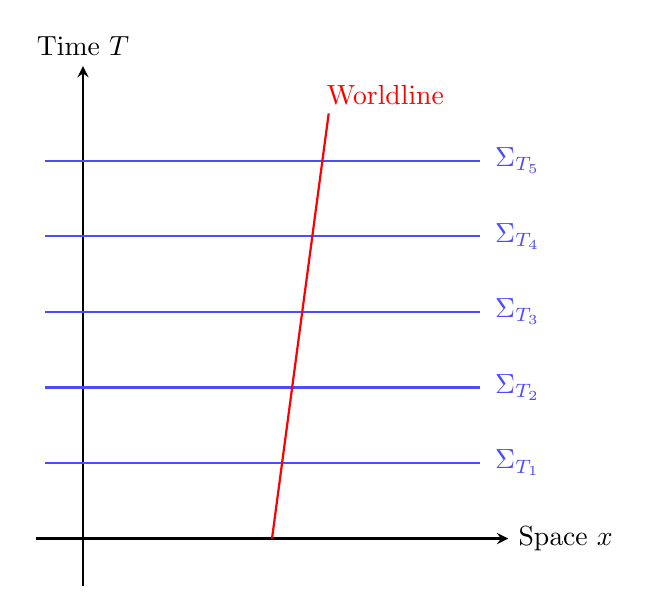
\begin{tikzpicture}[scale=1.2, >=stealth]
        % Axes
        \draw[->, thick] (-0.5,0) -- (4.5,0) node[right]{Space $x$};
        \draw[->, thick] (0,-0.5) -- (0,5) node[above]{Time $T$};

        % Foliation: horizontal lines (surfaces of constant time)
        \foreach \y in {0.8,1.6,2.4,3.2,4.0}
            \draw[blue!70, thick] (-0.4,\y) -- (4.2,\y);

        % Foliation labels
        \node[blue!70] at (4.6,0.8) {$\Sigma_{T_1}$};
        \node[blue!70] at (4.6,1.6) {$\Sigma_{T_2}$};
        \node[blue!70] at (4.6,2.4) {$\Sigma_{T_3}$};
        \node[blue!70] at (4.6,3.2) {$\Sigma_{T_4}$};
        \node[blue!70] at (4.6,4.0) {$\Sigma_{T_5}$};

        % A particle's worldline
        \draw[red, thick] (2,0) .. controls (2.2,1.5) and (2.4,3) .. (2.6,4.5);
        \node[red] at (3.2,4.7) {Worldline};
    \end{tikzpicture}
    \caption{A spacetime diagram illustrating the foliation of spacetime into hypersurfaces of constant universal time $\Sigma_T$ (blue lines). A physical object follows a timelike worldline (red curve) that passes through the sequence of universal 'nows'.}
    \label{fig:foliation}
\end{figure}

\begin{remark}[Calendar analogy]
The universal interval $\Delta T$ is like the change in date stamp (non-repeating, global order), while local labels $T_i=a_iT+b_i$ play the role of time zones/calendars. Physical ticks satisfy $d\tau=S\,dT$ (fewer ticks per unit $T$ for $S<1$), so clocks can disagree on elapsed ticks over the same date change, but not on the ordering supplied by $T$.
\end{remark}

\section*{Existence and Construction of the Universal Time Foliation}
\label{app:existence}
\begin{theorem}[Existence on cosmological domains]
\label{thm:existenceT}
Let $(M,g)$ be a time–orientable, globally hyperbolic spacetime region modeling the large–scale universe. Then the existence of a smooth \emph{time function} $T:M\to\mathbb{R}$ with timelike, future–directed gradient is guaranteed, and its level sets $\{\Sigma_T\}$ are spacelike Cauchy hypersurfaces (hence a $3{+}1$ foliation).
\end{theorem}

\begin{proof}[Sketch]
Global hyperbolicity implies the existence of smooth Cauchy time functions whose level sets are Cauchy hypersurfaces (classical results due to Geroch; Bernal–-S\'anchez). Thus the existence of a smooth $T$ with timelike $\nabla T$ is guaranteed, providing a foliation of $M$ by spacelike slices $\Sigma_T$. On cosmological domains well approximated by FLRW, this $T$ coincides (up to an additive constant and small inhomogeneous corrections) with standard cosmic time.
\end{proof}

\paragraph{Operational construction (CMB–anchored).}
To make $T$ empirical rather than merely existential, define the large–scale \emph{energy frame} $U^\mu$ as the timelike eigenvector of the coarse–grained stress–energy $\overline{T}^{\mu}{}_{\nu}$ (Landau–Lifshitz frame) on smoothing scales $L\gtrsim 100\,\text{Mpc}$ \emph{(exceeding the homogeneity/BAO scale and the size of the largest bound structures)}. Observationally, $U^\mu$ is the \emph{CMB rest frame} (vanishing dipole). When the vorticity of $U^\mu$ is negligible on these scales (consistent with current bounds), Frobenius’ theorem gives hypersurface–orthogonality. Then $T$ is \emph{constructed} by
\[
U[T]=1,\qquad T\big|_{\Sigma_0}=0,
\]
i.e.\ $T$ increases by one unit per unit proper time along the $U$-congruence, with initial slice $\Sigma_0$ (e.g.\ the big–bang surface in FLRW). In exact FLRW, this yields $T\equiv t_{\rm cos}+\text{const}$.

\paragraph{Geometric $3{+}1$ split induced by $T$.}
In $T$-adapted coordinates the metric reads
\[
ds^2=-N^2\,dT^2+h_{ij}\big(dx^i+N^i dT\big)\big(dx^j+N^j dT\big),
\]
with lapse $N>0$, shift $N^i$, spatial metric $h_{ij}$, and unit normal $n^\mu$ to $\Sigma_T$.

\begin{corollary}[Tick suppression from $T$]
\label{cor:suppression}
Let $u^\mu$ be the 4–velocity of any timelike worldline, and define the relative gamma by
\[
\gamma_{\rm rel}\;:=\;-u_\mu n^\mu\;\ge 1.
\]
Then the proper–time rate relative to the universal foliation satisfies
\[
\boxed{\;\frac{d\tau}{dT}\;=\;\frac{N}{\gamma_{\rm rel}}\;\equiv\;S(T,x)\;\le 1\;}.
\]
In particular: (i) flat, no gravity $N=1\Rightarrow d\tau/dT=\sqrt{1-v^2/c^2}$; (ii) static gravity at rest $v=0\Rightarrow d\tau/dT=\sqrt{-g_{00}}$ (weak field $\approx \sqrt{1+2\Phi/c^2}$); and (iii) in general the factors multiply.
\end{corollary}

\begin{proof}[One–line proof]
Decompose $u^\mu=\gamma_{\rm rel}(n^\mu+v^\mu)$ with $n_\mu v^\mu=0$ \emph{and $|v|$ the physical 3-speed measured by an Eulerian observer, i.e.\ $|v|^2=h_{ij}v^i v^j$}. Then $u\!\cdot\!n=-\gamma_{\rm rel}$ and, in the $3{+}1$ line element, $d\tau^2=N^2 dT^2 - h_{ij}(dx^i+N^i dT)(dx^j+N^j dT)$. Eliminating $dx^i$ via $u^\mu$ gives $d\tau/dT=N/\gamma_{\rm rel}$.
\end{proof}

\paragraph{Selection principles (optional uniqueness).}
To avoid arbitrariness among admissible time functions, one may \emph{select} $T$ by a geometric criterion:
\begin{itemize}
  \item \textbf{CMC/York time:} choose slices with constant mean curvature $K(T)=\text{const}$;
  \item \textbf{Harmonic time:} solve $\Box T=0$ with timelike $\nabla T$;
  \item \textbf{Minimal shear/twist:} minimize an action built from the shear/vorticity of the large–scale congruence.
\end{itemize}
Each reduces to standard cosmic time in FLRW and yields the same suppression law \(\,d\tau/dT=N/\gamma_{\rm rel}\).

\paragraph{Empirical pipeline}
\begin{enumerate}
  \item \textbf{Fix a smoothing scale} $L$ (e.g.\ $100$--$200$ Mpc) and construct the energy frame $U^\mu$ from CMB/large–scale structure (dipole–zero boosts).
  \item \textbf{Integrate} the transport equation $U[T]=1$ along the $U$-congruence with a chosen $\Sigma_0$ to obtain a field $T(x)$ on a $\Lambda$CDM background.
  \item \textbf{Validate isotropy on slices:} check that BAO/CMB anisotropy statistics are maximally isotropic on $\Sigma_T$ (consistency with comoving cosmic time).
  \item \textbf{Clock–rate checks:} for local systems with velocity $v$ and potential $\Phi$, verify that observed rates obey $f(T)=f_0\,\big(N/\gamma_{\rm rel}\big)$ (GPS, gravitational redshift, storage–ring clocks).
  \item \textbf{Bound residual vorticity:} quantify how small a nonzero twist of $U^\mu$ must be to spoil hypersurface–orthogonality; compare with observational limits from, e.g., \emph{Planck} Collaboration CMB isotropy/vorticity bounds \cite{PlanckVorticityConstraint,PlanckIsotropy2018}.
\end{enumerate}

\paragraph{Scope and limitations.}
The existence theorem applies on globally hyperbolic, cosmological domains; strong inhomogeneities or significant large–scale vorticity may require a foliation atlas $\{(U_a,T_a)\}$ with affine transition maps. Within its domain, the suppression law \(\,d\tau/dT=N/\gamma_{\rm rel}\) is a forced geometric projection, independent of clock microphysics (ideal Lorentz–respecting clocks).

\newpage


\section{Tick Suppression Without the Universal Time Field}
\label{sec:SuppNoT}

We work entirely within standard GR, assuming only the clock hypothesis (ideal clocks
advance by proper time) and a choice of \emph{reference observers} forming a timelike
congruence.

\begin{definition}[Reference congruence]
Let $n^\mu$ be any smooth, future–directed, unit timelike vector field ($n_\mu n^\mu=-1$),
interpreted as the 4–velocity field of a family of Eulerian observers. Let $\sigma$ denote
their proper time parameter along the integral curves of $n^\mu$.
\end{definition}

\begin{lemma}[Local decomposition and relative factor]
For any timelike worldline with 4–velocity $u^\mu$, decompose
\[
u^\mu=\gamma_{\mathrm{rel}}\!\left(n^\mu+v^\mu\right), \qquad
n_\mu v^\mu=0,\quad \gamma_{\mathrm{rel}}=-\,u_\mu n^\mu \ge 1,
\]
where $v^\mu$ is spatial with respect to $n^\mu$ (i.e.\ $n_\mu v^\mu=0) \,$and its magnitude
$|v|$ is the \emph{physical 3-speed} measured in the local rest frame of the $n^\mu$-congruence.
In an orthonormal tetrad with $e_{(0)}^\mu=n^\mu$, one has $u^{(0)}=\gamma_{\mathrm{rel}}$ and
$|v|^2=\delta_{ij}u^{(i)}u^{(j)}/\gamma_{\mathrm{rel}}^2$ (equivalently $|v|^2=h_{ij}v^i v^j$).
\end{lemma}

\begin{corollary}[Congruence–relative suppression]
\label{cor:SuppNoT}
The moving clock’s proper time rate relative to the reference observers’ proper time is
\begin{equation}
\boxed{\;\frac{d\tau}{d\sigma}=\frac{1}{\gamma_{\mathrm{rel}}}\;\le 1\;}
\qquad\text{\normalfont (Congruence–Relative Tick Suppression Law).}
\label{eq:CRTS}
\end{equation}
Thus, for any pair of co–located events compared by the reference observers,
an ideal clock with 4–velocity $u^\mu$ accumulates fewer ticks than the reference
(“slower clock”) by the factor $1/\gamma_{\mathrm{rel}}$.
\end{corollary}

\begin{proof}
Choose an orthonormal tetrad $\{e_{(a)}^\mu\}$ with $e_{(0)}^\mu=n^\mu$. Then
$u^{(0)}=\gamma_{\mathrm{rel}}$ is the time component of $u^\mu$ measured by the
reference observers. The clock hypothesis gives $d\tau$ as the clock’s invariant interval,
and the reference observers’ proper time increment is $d\sigma$. Standard time–dilation
in this local orthonormal frame yields $d\tau = d\sigma/\gamma_{\mathrm{rel}}$.
\end{proof}

\paragraph{Coordinate form (ADM, optional).}
If one introduces any time function $t$ whose constant–$t$ hypersurfaces are orthogonal
to $n^\mu$ (so $n^\mu$ is the unit normal) with lapse $N$ and shift $N^i$, then
\[
ds^2=-N^2 dt^2 + h_{ij}(dx^i+N^i dt)(dx^j+N^j dt),
\]
and the rate relative to $t$ is
\[
\frac{d\tau}{dt}
= \sqrt{N^2 - h_{ij}(v^i+N^i)(v^j+N^j)}
\;=\; \frac{N}{\gamma_{\mathrm{rel}}}\quad(\text{for }N^i=0).
\]
This reproduces the familiar factors: (i) flat, $N=1 \Rightarrow d\tau/dt=\sqrt{1-v^2/c^2}$;
(ii) stationary at rest, $v=0 \Rightarrow d\tau/dt=\sqrt{-g_{00}}$; (iii) in general, the
kinematic and gravitational factors multiply when $N^i=0$.

\paragraph{Remarks.}
(1) No global foliation or universal time is required: suppression is a \emph{local,
congruence–relative} statement encoded by $\gamma_{\mathrm{rel}}=-u\!\cdot\! n$.\\

\noindent
(2) Choosing the \emph{cosmic} congruence $n^\mu=U^\mu_{\rm CMB}$ and introducing its
orthogonal slicing recovers the universal–time projection law $d\tau/dt = N/\gamma_{\mathrm{rel}}$
as a special case.\\

\noindent
(3) Any ideal clock whose dynamics integrate over $d\tau$ (atomic transitions, oscillators,
decays) inherits the same suppression factor relative to the chosen reference observers.\\

\noindent
(4) \emph{Optional energy connection.} In the $n^\mu$-frame, a particle of rest mass $m$
has energy $E=-p_\mu n^\mu = m \gamma_{\mathrm{rel}} c^2$ and spatial momentum
$p^{\langle i\rangle}=m\gamma_{\mathrm{rel}} v^i$; the same $\gamma_{\mathrm{rel}}$ that enhances
$(E,\mathbf{p})$ suppresses $d\tau/d\sigma$ via \eqref{eq:CRTS}, aligning with the
mechanistic “energy–budget” narrative elsewhere in the paper.

\newpage

\section{Glossary of Symbols}
\vspace{-1.0em}
\begin{longtable}{p{0.15\linewidth} p{0.6\linewidth} p{0.15\linewidth}}
    \toprule
    \textbf{Symbol} & \textbf{Description} & \textbf{Units} \\
    \midrule
    \endfirsthead
    \toprule
    \textbf{Symbol} & \textbf{Description} & \textbf{Units} \\
    \midrule
    $T$ & The universal time coordinate. & s \\
    $dT$ & An infinitesimal increment of universal time. & s \\
    $\Sigma_T$ & A hypersurface of constant universal time $T$. & ---\footnote{Denotes "Not Applicable," used for concepts that are not physical quantities with units.} \\
    $U^\mu$ & The 4-velocity of the cosmic flow field. & Dimensionless (or m/s) \\
    $n^\mu$ & The unit vector field normal to the $\Sigma_T$ slices. & Dimensionless \\
    $N$ & The lapse function in the 3+1 formalism. & Dimensionless \\
    $N^i$ & The shift vector in the 3+1 formalism. & m/s \\
    $h_{ij}$ & The 3D spatial metric on a $\Sigma_T$ slice. & Dimensionless \\
    $S$ & The total suppression factor ($S = d\tau/dT$). & Dimensionless \\
    $\alpha$ & The relativistic conversion coefficient ($S=\alpha$ for ideal clocks). & Dimensionless \\
    $d\tau$ & An infinitesimal increment of proper time (duration). & s \\
    $\gammarel$ & The relativistic gamma (Lorentz) factor ($\alpha = 1/\gammarel$). & Dimensionless \\
    $v$ & Physical 3-velocity relative to Eulerian observers. & m/s \\
    $v_{\mathrm{pec}}$ & Peculiar velocity relative to the CMB frame. & m/s \\
    $\Phi$ & The Newtonian gravitational potential. & m$^2$/s$^2$ \\
    $g_{\mu\nu}$ & The 4D spacetime metric tensor. & Dimensionless \\
    $\mathcal{M}$ & The 4D spacetime manifold. & --- \\
    MCIF & Momentarily Comoving Inertial Frame. & --- \\
    CMB & Cosmic Microwave Background. & --- \\
    \bottomrule
\end{longtable}

\newpage

\begin{thebibliography}{99}

\bibitem{Einstein1905}
A.~Einstein,
``Zur Elektrodynamik bewegter Körper,''
\emph{Annalen der Physik} \textbf{17}, 891--921 (1905).

\bibitem{lorentz1952}
    Lorentz, H. A., Einstein, A., Minkowski, H., \& Weyl, H. (1952). \textit{The Principle of Relativity}. Dover Publications.

\bibitem{Minkowski1908}
H.~Minkowski,
``Raum und Zeit (1908),'' in \emph{The Principle of Relativity},
Dover (1952).

\bibitem{PlanckIsotropy2018}
Planck Collaboration, Y.~Akrami \emph{et al.},
\emph{Planck 2018 results. VII. Isotropy and statistics of the CMB},
Astronomy \& Astrophysics \textbf{641}, A7 (2020),
arXiv:1906.02552.

\bibitem{PlanckVorticityConstraint}
Planck Collaboration, P.~A.~R.~Ade \emph{et al.},
\emph{Planck 2015 results. XVIII. Background geometry and topology},
Astronomy \& Astrophysics \textbf{594}, A18 (2016),
arXiv:1502.01593.

\bibitem{Rindler2006}
W.~Rindler,
\emph{Relativity: Special, General, and Cosmological}, 2nd ed.,
Oxford University Press (2006).

\bibitem{Carroll2004}
S.~M.~Carroll,
\emph{Spacetime and Geometry: An Introduction to General Relativity},
Addison–Wesley (2004).

\bibitem{MichelsonMorley1887}
A.~A.~Michelson and E.~W.~Morley,
``On the Relative Motion of the Earth and the Luminiferous Ether,''
\emph{American Journal of Science} \textbf{34}, 333--345 (1887).

\bibitem{Lorentz1904}
H.~A.~Lorentz,
``Electromagnetic phenomena in a system moving with any velocity less than that of light,''
\emph{Proc. Roy. Neth. Acad. Arts Sci.} \textbf{6}, 809--831 (1904).

\bibitem{BerziGorini1969}
V.~Berzi and V.~Gorini,
``Reciprocity principle and the Lorentz transformations,''
\emph{Journal of Mathematical Physics} \textbf{10}, 1518--1524 (1969).

\bibitem{LevyLeblond1976}
J.-M.~L\'evy–Leblond,
``One more derivation of the Lorentz transformation,''
\emph{American Journal of Physics} \textbf{44}, 271--277 (1976).

\bibitem{Mermin1984}
N.~D.~Mermin,
``Relativity without light,''
\emph{American Journal of Physics} \textbf{52}, 119--124 (1984).

\bibitem{Ashby2003}
N.~Ashby,
``Relativity in the Global Positioning System,''
\emph{Living Reviews in Relativity} \textbf{6}, 1 (2003).

\bibitem{HafeleKeating1972a}
J.~C.~Hafele and R.~E.~Keating,
``Around–the–World Atomic Clocks: Predicted Relativistic Time Gains,''
\emph{Science} \textbf{177}, 166--168 (1972).

\bibitem{HafeleKeating1972b}
J.~C.~Hafele and R.~E.~Keating,
``Around–the–World Atomic Clocks: Observed Relativistic Time Gains,''
\emph{Science} \textbf{177}, 168--170 (1972).

\bibitem{PoundRebka1960}
R.~V.~Pound and G.~A.~Rebka Jr.,
``Apparent Weight of Photons,''
\emph{Physical Review Letters} \textbf{4}, 337--341 (1960).

\bibitem{Bailey1977}
J.~Bailey \emph{et al.},
``Measurements of relativistic time dilatation for positive and negative muons in a circular orbit,''
\emph{Nature} \textbf{268}, 301--305 (1977).

\bibitem{Chou2010}
C.~W.~Chou, D.~B.~Hume, T.~Rosenband, and D.~J.~Wineland,
``Optical clocks and relativity,''
\emph{Science} \textbf{329}, 1630--1633 (2010).

\bibitem{Will2014}
C.~M.~Will,
``The Confrontation between General Relativity and Experiment,''
\emph{Living Reviews in Relativity} \textbf{17}, 4 (2014).

\bibitem{Noether1918}
E.~Noether,
``Invariante Variationsprobleme,''
\emph{Nachrichten von der Gesellschaft der Wissenschaften zu G\"ottingen, Mathematisch–Physikalische Klasse}, 235--257 (1918).
[Eng. trans.: \emph{Transport Theory and Statistical Physics} \textbf{1}, 186--207 (1971).]

\end{thebibliography}

\end{document}
